%(*[[header*)
\documentclass[doublespacing]{narfront}
% \documentclass{narfront} % single space

%   Dr. Thomas D. Schneider
%   National Cancer Institute
%   Laboratory of Experimental and Computational Biology
%   Frederick, Maryland  21702-1201
%   toms@ncifcrf.gov
%   permanent email: toms@alum.mit.edu (use only if first address fails)
%   http://www.lecb.ncifcrf.gov/~toms/

% SPECIAL DEFINITIONS

\newcommand{\theversion}{{version = 2.19 of fff.tex 2005 Feb 5
% 2005 Feb  5, 2.19: update references, MOCO
% 2003 Oct 19, 2.18: submitted version
}}

% % TEMPORARY PAGE SIZE DEFINITIONS
% these are now in elsartUSA
% % These make the pages have 1 inch margins, which prints better here
% % in the stupid USA.  I sure wish we would go metric!
% % \textheight 9.0 in % this works
% \textheight 9.0 in % this works
% % \topmargin 0.0 in % -0.5 would shift the whole thing up
% \topmargin 0.25 in % -0.5 would shift the whole thing up
% \headheight 0 in
% \headsep 0 in
% \textwidth 6.5 in
% % \oddsidemargin 0.25 in
% \oddsidemargin 0 in

% \textwidth 6.0 in

\newcommand{\runningtitle}{Fis Flip-Flops}

% \input general.definitions
\newcommand{\commentout}[1]{}
\newcommand{\todo}{\rule{0.5em}{1ex}}
% bold face around text with todo mark \todobf{text}
\newcommand{\todobf}[1]{{\rule{0.5em}{1ex}\textbf{ #1}}}
\newcommand{\fig}[1]{Fig.~\ref{#1}} % figure referencing mechanism
%% figure margin pointer:
\newcommand{\figmargin}[1]{\marginpar{\textcolor{blue}{$\Leftarrow$Fig \ref{#1}}}}
\newcommand{\bamhi}{{\emph{Bam}HI}} % a restriction enzyme
\newcommand{\ecori}{{\emph{Eco}RI}} % a restriction enzyme
\newcommand{\degrees}{${}^{\circ}$}
\newcommand{\degreesC}{${}^\circ \mbox{C}$}
\newcommand{\ribl}{\riw(b,l)}
\newcommand{\riw}{R_{iw}}

% Make a superscripted trademark.
% 2003 Aug 27:
% http://web.mit.edu/rsi/www/2003/help/faq/latex/#faq2
% 2. How do I put in a trademark/registered/copyrighted sign in LaTeX?
%             \textregistered for (R)
%             \copyright for (C)
%             \texttrademark for (TM)
\newcommand{\trademark}{${}^{\mbox{\scriptsize\textregistered}}$}
% old method:
% \newcommand{\trademark}{${^{\bigcirc \!\!\!\!\!\mbox{\tiny R}}}$}

\newcommand{\rsequence}{R_{sequence}}
\newcommand{\rfrequency}{R_{frequency}}

% The format of this file was starting from:
% Template article for preprint document class `elsart'
% SP 2001/01/05

% Use the option doublespacing or reviewcopy to obtain double line spacing
% \documentclass[doublespacing]{elsart}

% if you use PostScript figures in your article
% use the graphics package for simple commands
\usepackage{graphics}
% or use the graphicx package for more complicated commands
% \usepackage{graphicx}
% or use the epsfig package if you prefer to use the old commands
% \usepackage{epsfig}

% The amssymb package provides various useful mathematical symbols
\usepackage{amssymb}

% allow creation of html:
% latex2html package:
% http://www-texdev.mpce.mq.edu.au/l2h/docs/manual/
% \usepackage{html}
\newcommand{\latex}[1]{#1} % fake command for now
\newcommand{\html}[1]{{ }} % fake command for now THE SPACE IS NEEDED
\newcommand{\htmladdnormallink}[1]{{ }} % fake command for now THE SPACE IS NEEDED
% ********************************************************************************
% However this had some kind of conflict with the names in the elsevier
% package.  As soon as I call:
% 
% \usepackage{html}
% 
% I get:
% 
% ! LaTeX Error: No counter 'part' defined.
% 
% See the LaTeX manual or LaTeX Companion for explanation.
% Type  H <return>  for immediate help.
%  ...
% 
% l.495 \newcounter{lchapter}[part]
% 
% ?
% ! Emergency stop.
%  ...
% 
% l.495 \newcounter{lchapter}[part]
% 
% ********************************************************************************

\usepackage{color}

\begin{document}

\begin{frontmatter}

% Title, authors and addresses

% use the thanksref command within \title, \author or \address for footnotes;
% use the corauthref command within \author for corresponding author footnotes;
% use the ead command for the email address,
% and the form \ead[url] for the home page:
% \title{Title\thanksref{label1}}
% \thanks[label1]{}
% \author{Name\corauthref{cor1}\thanksref{label2}}
% \ead{email address}
% \ead[url]{home page}
% \thanks[label2]{}
% \corauth[cor1]{}
% \address{Address\thanksref{label3}}
% \thanks[label3]{}

\title{Molecular Flip-Flops Formed by Overlapping Fis Sites}
%23456789 123456789 123456789 123456789 123456789 123456789 123456789 123456789
%        1         2         3         4         5         6         7         8

% use optional labels to link authors explicitly to addresses:
% \author[label1,label2]{}
% \address[label1]{}
% \address[label2]{}
% \author{}
% \address{}

% original
% \author[label1,label2]{Paul N. Hengen},
% \author[label1]{Ilya G. Lyakhov},
% \ead{ilyakhov@ncifcrf.gov}
% \author[label3]{Lisa E. Stewart},
% \ead{stewartl@alkami.com}
% \and
% \author[label4]{Thomas D. Schneider\corauthref{cor}}
% \corauth[cor]{Corresponding author.}
% \ead{toms@ncifcrf.gov}
% \ead[url]{http://www.lecb.ncifcrf.gov/$\sim$toms/}

\author[label1,label2,label5]{Paul N. Hengen},
\author[label1,label5]{Ilya G. Lyakhov},
\ead{ilyakhov@ncifcrf.gov}
\author[label3]{Lisa E. Stewart},
\ead{stewartl@alkami.com}
\and
\author[label4,label6]{Thomas D. Schneider\corauthref{cor}}
\corauth[cor]{Corresponding author.}
\ead{toms@ncifcrf.gov}
\ead[url]{http://www.lecb.ncifcrf.gov/$\sim$toms/}

\address[label1]{Intramural Research Support Program, SAIC, NCI Frederick,
Frederick, MD, USA}

\address[label2]{Current address:
Applied Biosystems, 3833 North First Street,
San Jose, CA, 95134-1701, USA}

\address[label3]{Volunteer to the National Cancer Institute at Frederick.
Current address:
Alkami Biosystems, Inc.
P.O. Box 11216,
Berkeley, CA 94712-2216, USA}

\address[label4]{
Laboratory of Experimental and Computational Biology,
National Cancer Institute at Frederick,
P. O. Box B, Building 469, Room 144,
Frederick, MD  21702-1201, USA,
301) 846-5581 (-5532 for messages),
fax: (301) 846-5598.
}

\address[label5]{
These authors contributed equally.
}

\address[label6]{
   The publisher or recipient acknowledges the right of the U.S. Government
   to retain a nonexclusive, royalty-free license in and to any copyright
   covering the article.
}

\begin{abstract}
% Text of abstract
\textbf{ % Abstract section
%(*]]header*)
The DNA binding protein Fis
frequently uses pairs of sites 7 or 11 base pairs apart.
Two overlapping Fis
sites separated by 11 base pairs are found in the
\emph{E. coli}
origin of
chromosomal replication.
Only one of these sites is bound by Fis at a time,
so the structure is a molecular flip-flop
that could
direct alternative firing of replication complexes in opposite directions.
Alternatively, the flip-flop could represent
part of an on-off switch for replication.
Because they can be used to create precise switched states,
molecular flip-flops could be used as the basis of a
novel molecular computer.
%(*[[text*)
}
\end{abstract}

\begin{keyword}
% keywords here, in the form: keyword \sep keyword
% \emph{Key words}:
% % 5, in alphabetical order: \\
Fis DNA binding
\sep
\emph{oriC}
\sep
flip-flop
\sep
information theory
\sep
sequence walker

% PACS codes here, in the form: \PACS code \sep code
% \PACS  % apparently does not apply to the Journal of Molecular Biology
\end{keyword}

\end{frontmatter}

\bibliographystyle{nar}

\theversion \\
running title: \runningtitle

% main text
% \section{}
% \label{}

% The Appendices part is started with the command \appendix;
% appendix sections are then done as normal sections
% \appendix

%*******************************************************************************
%* End of Front Matter *********************************************************
%*******************************************************************************

% \newpage

\section*{Introduction}

Fis is a well characterized site-specific DNA binding protein
which is known to bend DNA
and is involved in many site-specific recombination systems
\cite{Johnson.Simon1987}.
In addition, it autoregulates its own promoter
and activates other promoters
\cite{Finkel1992,Finkel1992.erratum}.
When \emph{Escherichia coli} encounters a rich
nutritional medium, the number of Fis molecules
increases from nearly zero to 25,000-50,000 dimers
per cell
\cite{Ball1992}.
Estimates of the number of Fis sites in the
\emph{E. coli} genome based on the average information
in Fis sites give a similar number, indicating that
most Fis molecules are controlling genetic
systems throughout the genome
\cite{Hengen.fisinfo,Travers.Muskhelishvili2001,Ussery.Brunak2001,Dorman.Deighan2003}.

Information analysis of Fis binding sites
and their surrounding sequences
has revealed previously unidentified
sites adjacent to known ones
\cite{Hengen.fisinfo}.
We observed that pairs of Fis sites are often separated
by 7 or 11 bases in many genetic systems
\cite{Hengen.fisinfo,Schneider.Mastronarde.malign}.
These
Fis sites
often overlap
the binding sites of other proteins
in biologically significant places such as
the Xis site of
$\lambda$ \emph{att}
\cite{Schneider.walker},
\emph{dif},
\emph{nrd},
\emph{ndh}
and the
\emph{fis} promoter (data not shown).
To understand the
significance of these pairs
we sought to determine whether Fis binds cooperatively
or antagonistically at the adjacent sites.
In this study we show that
in artificial DNA constructs,
overlapping Fis sites 7 or 11 base pairs apart
cannot be bound simultaneously
and therefore act as a molecular flip-flop.

DNA replication starts at 84.6 minutes on the
circular \emph{E. coli} K-12 chromosome
at a locus called \emph{oriC} \cite{Messer.Weigel1996,Baker.Bell1998}.
Bidirectional replication starting at
\emph{oriC}
\cite{Prescott.Kuempel1972,Bird.Caro1972}
is completed in the terminus region
half way around the chromosome \cite{Hill1996}.
Replication is dependent on the DnaA protein,
which binds at 5 sites in 
\emph{oriC}.
Using sequence 
walkers
\cite{Schneider.walker},
we observed that there are likely to be two
Fis sites 11 base pairs apart
wedged precisely between two of the DnaA sites.
We show that these sites are not bound simultaneously.

%* **************************************************************************

\section*{Materials and Methods}

\subsection*{Sequence analysis programs}

Delila system programs were used
for handling sequences and information calculations
\cite{Schneider1982,Schneider1984,Schneider1986,Schneider.Stephens1990,Stephens.Schneider.Splice,Schneider.Ri,Schneider.walker}.
Figures were generated automatically
from raw GenBank data using Delila and UNIX
script programs.
Further information is available at
http://www.lecb.ncifcrf.gov/$\sim$toms/.

\subsection*{Design of Fis binding experiments}

Synthetic DNAs containing
strong Fis sites separated by 11 and 7 base pairs were designed
by selecting from the most frequent bases at each position in the
Fis sequence logo
\cite{Hengen.fisinfo}.
These were then merged
with the same sequence shifted by 11 or 7 base pairs
by comparing the $\ribl$ values for various choices.
(Note: the consensus sequence of the early model we used
was TTT\underline{G}(G/C)TCAAA\underline{A}TTTGA(G/C)\underline{C}AAA
which differs from
that of the logo
\cite{Schneider.Zen2002}.
The $0$ and strongly conserved $\pm 7$ positions are underlined.)
Five extra bases were added to the ends based on the natural
sequences around the \emph{hin}
proximal and medial sites
for the overlap 11 oligo,
and
the sequences around \emph{cin}
external and proximal sites
were used for the overlap 7 oligo \cite{Hengen.fisinfo}.
The DNAs were made self complementary
(\fig{fig.sequences-overlap}a, b).
Sites separated by 23 bases were created starting with the 11 base
separated DNA and duplicating the central overlap region.
A \bamhi\ site was also inserted
and the DNA was flanked by \ecori\ sites
(\fig{fig.sequences-overlap}c).
Oligos were synthesized
with biotin on the $5'$ end
and gel purified
(Oligos Etc., Wilsonville, OR, USA).
To ensure thorough annealing, they were heated to
90\degreesC\ for 10 minutes,
and slowly cooled to room temperature.
The annealed products were electrophoresed through
an 8\% (w/v) polyacrylamide gel, and the bands corresponding
to the linear duplex DNA of the correct size were
sliced from the gel.  DNA was recovered by
electroelution and extracted with isoamyl alcohol to
remove ethidium bromide.
A non-specific control DNA
was composed of the two 66 bp \emph{Hin}FI
fragments from bacteriophage $\phi$X174
(Life Technologies, Inc.).
This DNA did not shift even at the highest concentration of Fis used.
Gel mobility shift experiments were performed
as described previously,
using chemiluminescent detection
\cite{Hengen.fisinfo}.
Fis used in the experiment shown in
\fig{fig.gel-overlap}
was a gift from Reid Johnson.

Hairpin DNA oligos containing the
\emph{oriC} region
(\fig{fig.oriCexperiment})
were synthesized with a
% hyphenation of tetramethylrhodamine is needed:
$5'$-tetra\-methyl\-rhodamine modification and gel purified (Oligos Etc.).
By using a hairpin, an annealing step is not required and the
oligos are exactly equimolar
\cite{Hengen.fisinfo}.
Horizontal 8\% PAGE was used for the gel mobility shift assay and band positions
were visualized with a FMBIO II fluorescent scanner (Hitachi) with an
excitation wavelength of
532 nm and detection at 605 nm.

\subsection*{Fis protein isolation}

For the experiment shown in \fig{fig.oriCexperiment},
Epicurian Coli\trademark\
BL21-Gold(DE3) cells
(Stratagene) \cite{Studier1986},
transformed with pRJ1077 plasmid
(a gift from Reid Johnson)
were used for Fis protein isolation by modification of a previous method
\cite{Pan.Johnson1996}.
A 10 ml overnight culture was added to 1 l of SOB media, shaken at 37\degreesC\
for 2 hours 30 minutes, induced by 1 $\mu$M
isopropyl-$\beta$-D-thiogalactopyranoside
(IPTG)
and shaken again for 1 hour.  The culture was centrifuged and the cell
pellet was resuspended in 50 ml FLBC buffer (50 mM Tris-HCl pH 7.5, 10 mM
EDTA), containing 200 mM NaCl and 0.1 mM
phenylmethylsulfonyl fluoride
(PMSF), sonicated with a Cole-Parmer
Ultrasonic Processor model CP 70T 3 times for 10 minutes (40W) on ice and
centrifuged at 2000 g for 20 minutes.  The supernatant was loaded on a 10 ml
Q-Sepharose\trademark\ Fast Flow (Amersham Pharmacia Biotech) column equilibrated
with the same buffer and washed with 10 ml of FLBC buffer containing 300 mM
NaCl.  Flow-through and wash fractions were combined and the mix was loaded
on a 10 mL Heparin Sepharose\trademark\ CL-6B (Amersham Pharmacia Biotech), washed
with 50 ml of FLBC buffer, containing 300 mM NaCl and eluted with a 100-ml
300-2000 mM NaCl gradient of FLBC buffer. Fractions were analyzed by
SDS-electrophoresis.

\subsection*{Molecular Models of Fis Binding to DNA}

% Lisa E. Stewart, Paul N. Hengen, and Thomas D. Schneider

In order to understand the sequence logo for Fis binding sites
\cite{Hengen.fisinfo},
we constructed three dimensional models of Fis-DNA binding.
The models of Fis interacting
with DNA
were built using
Insight II software
from Biosym Technologies, Inc.,
on an IRIS computer
(Silicon Graphics, Inc.),
and displayed with RasMol 2.5, available at
\\
\latex{http://molbiol.soton.ac.uk/rasmol.html}
\html{{\htmladdnormallink
{http://molbiol.soton.ac.uk/rasmol.html}
{http://molbiol.soton.ac.uk/rasmol.html}}}
\\
or
\\
\latex{ftp://ftp.dcs.ed.ac.uk/pub/rasmol/}
\html{{\htmladdnormallink
{ftp://ftp.dcs.ed.ac.uk/pub/rasmol/}
{ftp://ftp.dcs.ed.ac.uk/pub/rasmol/}}}.
\\
The Fis protein coordinates are those of the
Protein Data Bank
\\
(%
\latex{http://www.rcsb.org/pdb/}%
\html{{\htmladdnormallink
{http://www.rcsb.org/pdb/}
{http://www.rcsb.org/pdb/}}})
entry
\latex{1fia}%
\html{{\htmladdnormallink
{1fia}
{http://www.rcsb.org/pdb/cgi/explore.cgi?pid=11784981339478&pdbId=1FIA}}}.

In Fis-DNA models built by earlier workers
either B-form DNA with no particular base sequence was smoothly
bent and placed next to the X-ray crystal model of Fis
\cite{Kostrewa1991,Kostrewa1992},
or the single distal \emph{hin}
Fis binding site (V01370, 180, 8.9 bits)
was used and kinks added to the DNA
at positions based
on the DNase I hypersensitive pattern \cite{Yuan1991}.
Since the sequence logo gives a detailed model for the
sequence conservation at Fis sites, we used this
information to construct three models:

\begin{itemize}
\item
a single Fis homodimer binding to the consensus sequence as
determined by the logo
% \begin{rawhtml}
% <a href = "#fig1">figure 1</a>
% \end{rawhtml}
(\latex{\fig{fig.fismodels}A}).

\item
two Fis homodimers binding to two Fis sites spaced 11 base
pairs apart on DNA
% \begin{rawhtml}
% <a href = "#fig2">figure 2</a>
% \end{rawhtml}
(\latex{\fig{fig.fismodels}B}).

\item
two Fis homodimers binding to two Fis sites spaced 7 base
pairs apart on DNA
% \begin{rawhtml}
% <a href = "#fig3">figure 3</a>
% \end{rawhtml}
(\latex{\fig{fig.fismodels}C}).

\end{itemize}

We used several criteria for making the first model.
As noted by previous workers,
Arg85 and Lys91 in the D helix
are likely to be involved in DNA binding
since mutations at these amino acids
interfere with DNA binding
\cite{Kostrewa1991,Kostrewa1992}.
The logo shows highly conserved G-C base pairs at $-7$ and $+7$
in major groove positions, as is common
when contacts are made by proteins
with helix-turn-helix motifs
\cite{Yuan1991,Papp.helixrepa}.
In addition, methylation of these bases blocks Fis from binding
\cite{Bruist1987} and Fis protects these bases against methylation
\cite{Thompson1987}.
However, as mentioned in previous studies,
with B-form DNA, the Gs at
$ \pm 7$
would be further apart than the distance
between the two DNA-contacting D helices of Fis.
Fis can deflect DNA from 40 to 90\degrees\
\cite{Finkel1992,Kostrewa1991,Yuan1991,Thompson.Landy1988},
so we can attain
a shorter distance between the two DNA contact points at $\pm 7$
either by
`bending' (a gradual curvature of the helix axis over a sequence of more than
two bases) or by `kinking' (a sharp change in the DNA strand's axial
direction between two adjacent bases)
at one or more locations between the two contacts
\cite{Wu.Crothers1984}.

If specific contacts are not formed,
a smoothly bent DNA might be expected to produce smooth sequence
conservation over the binding region, but
the logo shows strong
variable 
conservation of base sequences at positions -5 through +5,
so
it is likely that
the deflections are not smooth.
Furthermore,
both
CA and TG, which are conserved at positions
$-4$ to $-3$ and $+3$ to $+4$
\cite{Kostrewa1992}
(\emph{i.e.} positions $\pm 3.5$), have been
shown to display unusually large roll (rotation about the long axis
between base pairs
\cite{Dickerson1989}).
The CRP-DNA complex displays a
90\degrees\ bend that results from CA and TG kinking
\cite{Barber1990,Schultz1991}
(see
Papp \emph{et al.}
\cite{Papp.helixrepa}
for the CRP sequence logo).

Additionally,
the other two pyrimidine-purine (Py-Pu)
base sequences conserved in Fis sites, TA \cite{Goodsell1994} and
CG \cite{Gorin1995,Suzuki.Yagi1995,Crothers.Nadeau1990,Cognet1995},
show this high-roll characteristic.
These four kinking dinucleotides appear frequently
at $\pm 3.5$ and $\pm 7.5$.
They account for
the base frequencies in the logo and they identify kink locations
which could result in the observed DNA deflection \cite{Lazarus1993}.
Examination of the individual
Fis binding sites confirms this observation.
With the exception of seven
Fis sites in our set:
\emph{fis} X62399 292,
\emph{nrd} K02672 3266,
\emph{aldB} L40742 153,
\emph{hin} V01370 68,
\emph{cin} X01828 289,
\emph{gin} M10193 389,
and
\emph{hns} X07688 655,
sites
which do not have a Py-Pu step at $\pm 3.5$
do have one displaced just one position left or right \cite{Barber1990}.
In addition, these Py-Pu kinks form during energetic minimization
of a Fis-DNA complex \cite{Sandmann1996}.
We therefore constructed our model using
two 42\degrees\ kinks at $\pm 3.5$.
More kinking would prevent Fis from fitting into
the two successive major grooves.
Two 50\degrees\ kinks were also added at positions $\pm 7.5$
because this was the largest observed kink found
for CAP protein binding \cite{Schultz1991}.

% \begin{enumerate}
% \item \emph{fis} X62399 292,
% \item \emph{nrd} K02672 3266,
% \item \emph{aldB} L40742 153,
% \item \emph{hin} V01370 68,
% \item \emph{cin} X01828 289,
% \item \emph{gin} M10193 389,
% \item \emph{hns} X07688 655,
% \end{enumerate}

The midsection of the logo is AT rich
and this should create a higher twist,
leading to a compression in the minor groove
\cite{Wu.Crothers1984,Lipanov.Chuprina1987,Kostrewa1992}.
We incorporated this compression into our model
by making the helical repeat through the central A-T tract
(bases $-2$ to $+2$)
10 base pairs per turn
and setting the remainder of the model to
10.6 base pairs per turn for B-form DNA
\cite{Peck1981,Rhodes1980,Rhodes1981}.

We tried to maximize the overall DNA bend angle of Fis bound
to DNA and found that the best we could do,
while avoiding stereochemical collisions, was 60\degrees.
This model of a single Fis homodimer contacting DNA
\html{(figure 1)}%
\latex{ (\fig{fig.fismodels}A) }
has two kinks and one compression
that allow
the four nitrogens of Arg85
to be within contact distance ($<3.5$ \AA)
of either the O6 or N7 acceptor of
each G at
$\pm 7$
and Lys91 to be within 3.5 \AA\
of the phosphate backbone at $\pm 1.5$
with no major structural conflicts.

% \begin{rawhtml}
% <a name="fig1"></a>
% <IMG SRC="../fismono.gif">
% <BR>
% Figure 1.
% Molecular model of a single Fis dimer binding to DNA.
% \end{rawhtml}

To investigate the consequences of two Fis
molecules binding to nearby sites,
we constructed 3 dimensional models with
Fis sites separated by 11 or 7 base pairs.
For the two overlapping Fis models, we extended the general scheme
of modeling a Fis homodimer
to the synthetic DNA sequences
used in our gel shift experiment.

For the overlap 11 model
\html{(figure 2),}%
\latex{(\fig{fig.fismodels}B),}
different kinks from the two adjacent sites would be in the same
place.
Because 50\degrees\ kinks would prevent Fis from fitting into either site,
we made both 42\degrees.
We incorporated 50\degrees\ kinks
on the outside two positions, as in the
single site model.  We also increased the twist to $-36$\degrees\ at
all A-T pairs within the central region
\cite{Goodsell1994}.

% \begin{rawhtml}
% <a name="fig2"></a>
% <IMG SRC="../dbl11.gif">
% <BR>
% Figure 2.
% Molecular model of two Fis dimers binding to Fis sites separated
% by 11 base pairs.
% \end{rawhtml}

For the overlap 7 model
\html{(figure 3),}%
\latex{(\fig{fig.fismodels}C),}
the two outside TG and CA ends were kinked
50\degrees\ to conform to the single Fis model.  However, two pairs which would
normally be kinked were not Py-Pu pairs in this sequence.  We excluded kinking
of the left site at $\pm 7.5$ due to a Py-Py pair (CT) and we excluded kinking of
the right site at $-7.5$ due to a Pu-Pu pair (AG).
Therefore, we only added
42\degrees\ kinks at three positions: at two Py-Pu pairs (left $-3.5$ CA and
right $+3.5$ TG) which correspond to the single Fis model, and
at one in the center (TA).
As in the overlap 11 model,
twists of $-36$\degrees\ were made throughout any A-T tract
to be consistent with the single homodimer model.

% \begin{rawhtml}
% <a name="fig3"></a>
% <IMG SRC="../dbl07.gif">
% <BR>
% Figure 3.
% Molecular model of two Fis dimers binding to Fis sites separated
% by 7 base pairs.
% \end{rawhtml}

We found that two Fis
proteins separated by 11 base pairs would strongly interpenetrate.
On the other hand, two Fis proteins separated by 7 base pairs have a
minimal van der Waals force conflict between the two central D helices,
but this might be accommodated for by flexibility
of the DNA-protein complex.
Given that the D helices cannot fit directly into B-form DNA,
there is some uncertainty as to how Fis binds DNA.
We thought
that 11-base separated Fis
molecules
\html{(figure 2)}%
\latex{(\fig{fig.fismodels}B)}
would compete for binding but that a 7-base separation
\html{(figure 3)}%
\latex{(\fig{fig.fismodels}C)}
might allow
simultaneous binding.

%********************************************************************************
%********************************************************************************
%********************************************************************************

\section*{Results and Discussion}

\subsection*{Fis site structures suggest self-competition}

In a previous study we used 60 experimentally defined
Fis binding sites to construct a highly detailed and reliable
model of Fis binding to DNA
\cite{Hengen.fisinfo}.
When we searched DNA sequences for Fis sites
using
this
information-theory based weight matrix model,
we observed
Fis sites spaced 11 base pairs apart in
the DNA inversion systems
\emph{hin}, \emph{gin}, and \emph{min}
(see Fig. 5 in Hengen \emph{et al.} \cite{Hengen.fisinfo}).
A search of the entire \emph{E. coli} genome
shows that Fis sites are frequently separated by 11 bases
(\fig{fig.genomescan}).\figmargin{fig.genomescan}
Although the same number of sites is found in a genome-sized
equiprobable random sequence,
this does not mean that the sites are not functional.
Many binding sites have just the amount of information
($\rsequence$)
needed for them
to be found in the genome
($\rfrequency$)
\cite{Schneider1986}.
According to Shannon's principles
\cite{Shannon1948},
a well-coded communications system looks like random noise from the
outside,
and Fis site pairs may follow this principle.
So the spike of sites coming in pairs is caused by the pattern
of Fis itself; it is intrinsic to the Fis model.
We cannot tell if
the pattern evolved because Fis sites were required to overlap
or whether
Fis sites overlap because the pattern evolved.
The peaks of Fis sites every three bases
in the genomic scan come from protein coding effects.
The peak of
spacing at 8 bases and
excess sites at
spacings of 1 and 3 bases were only
noticed during revisions of this paper; we do not understand
their significance.

Since B-form DNA twists every 10.6 base pairs,
the sites,
spaced 11 bp apart,
should be on the same side of the DNA.
While it is possible for two adjacent proteins
to bind simultaneously by a subtle interleaving of their DNA contacts,
as in the case of RNA polymerases
\cite{Goodrich.McClure1991,Strainic.deHaseth2000},
it seems more likely that
in this case
they will compete for binding in the major groove
since, after an 11 base shift,
the sequence logo shows that the predominant G at $-7$ corresponds
to the G at +4 and the C at $-4$ corresponds
to the C at $+7$
(red arrows in \fig{fig.selflogo}).\figmargin{fig.selflogo}
Competition between these internally redundant patterns
\cite{Schneider.Mastronarde.malign}
would allow Fis to change
the point at which the DNA is bent.
Perhaps this is important for inversion.

In contrast to the 11 base spacing described above,
in bacteriophage P1 \emph{cin},
bacteriophage P7 \emph{cin},
\emph{E. coli e14 pin} sites,
and in the genome scan
(\fig{fig.genomescan}),
pairs of Fis sites are observed at spacings of
7 bases.
This would place the Fis dimers
122\degrees\/
apart on B-DNA
($ 360\mbox{\degrees} - 
360\mbox{\degrees}
\mbox{ per turn}
\times 7 \mbox{ bases}
/
10.6 \mbox{ bases per turn}
= 122\mbox{\degrees}
) $.
After a 7 base shift, the sequence logo shows
that the predominant G at $-7$ would match the A/T/g/c
of the minor groove on the opposite
face of the DNA at coordinate 0, while the C/T at $-4$ would match the T/C at
$+3$ and the A/G at $-3$ would match the G/A at $+4$
(green arrows in \fig{fig.selflogo}).
This allows for the possibility that the
two proteins bind at the same time,
which might also be important to the
function of these regions.

To investigate the consequences of two Fis
molecules binding to nearby sites,
we constructed 3 dimensional models
(\fig{fig.fismodels}).\figmargin{fig.fismodels}
We found that two Fis proteins
bound to sites separated by 11 base pairs might strongly interpenetrate.
In contrast, a 7 base pair separation might only have a
minimal van der Waals force conflict between the two central D helices.
This might be accommodated for by flexibility
of the DNA-protein complex,
given that
there is some uncertainty as to how Fis binds DNA.
% We thought
The models suggest
that 11-base separated Fis
molecules would compete for binding but that a
7-base separation might allow
simultaneous binding.

These ideas are supported by the
preliminary observation that
synthetic DNA containing either
the \emph{hin} proximal or medial Fis sites
are bound by Fis in
electrophoretic mobility gel shift assays
\cite{Hengen.fisinfo}.
When these overlapping sites
were together on the same fragment
with a spacing of 11 bases,
only one band shift was observed,
suggesting that only one of the sites can
be bound at a time.
To test whether this is the case
requires using high concentrations of Fis
and strong Fis sites to ensure that both sites
would be bound if that were possible.

\subsection*{Test of the self-competition model}

To determine whether overlapping Fis sites
can be simultaneously bound by Fis,
we synthesized self-complementary DNA oligos with
strong Fis sites that
overlap by either 7 or 11 base pairs
(\fig{fig.sequences-overlap}a,b)\figmargin{fig.sequences-overlap}
or that were separated by 23 base pairs
(\fig{fig.sequences-overlap}c)
and tested
their properties by gel shift.
Neither the 11 nor the 7 overlapping sites
showed a doubly-shifted band, even at an extremely high Fis/DNA ratio
and with exceptionally strong ($>12$ bits) Fis binding sites
(\fig{fig.gel-overlap}),\figmargin{fig.gel-overlap}
suggesting that only one Fis molecule could bind
to each DNA fragment.
The DNA fragment with two Fis sites separated by 23 base pairs
did double shift (\fig{fig.gel-overlap}),
demonstrating that two well separated Fis sites
can simultaneously bind two Fis molecules.
However, Fis can create a ladder of complexes
on non-specific sequences
\cite{Betermier1994}, and this might account for the double-shifts.
Under our conditions with short DNAs,
a non-specific
(all positions $< 1$ bit)
66 bp DNA fragment barely shifted
at high Fis concentration
(data not shown),
so the secondary shifts were not from non-specific binding.
These results demonstrate that Fis sites separated by 7 or 11 bases
cannot be bound simultaneously.

\subsection*{Genetic implications of Fis flip-flops}

The \emph{Escherichia coli} \emph{tyrT} promoter has
three Fis sites separated by 20 and 31 base pairs.
This separation corresponds to
our 23 base pair separated control experiment
(\fig{fig.sequences-overlap} and \fig{fig.gel-overlap}),
in which two Fis molecules bind independently.
The separation
in \emph{tyrT} is sufficient for three Fis dimers
to simultaneously position themselves on the same face of the DNA
to cooperatively bind
an $\alpha$CTD
subunit
and activate transcription of stable RNA promoters
\cite{Muskhelishvili1995}.
In addition to this activation mechanism,
which is based on separated sites,
Fis may also have evolved another control mechanism
that uses overlapping sites.

When we scanned our Fis individual information model across
various sequences,
we discovered
7 and 11 spacings at
DNA inversion regions,
the \emph{fis},
\emph{nrd},
and \emph{ndh} promoters, 
and at
\emph{dif},
\emph{E. coli oriC}
and
$\lambda$ \emph{att}
\cite{Schneider.walker,Hengen.fisinfo}.
In the latter three systems,
sequence walkers for
Fis sites overlap binding sites of other
proteins in biologically significant places,
so we do not think
that Fis sites appear at this spacing merely because
of the internal redundancy of the site.
Scanning with the Fis weight matrix also reveals two
strong Fis sites previously identified in \emph{oriC}
at coordinates
202 and 213
although only one was thought to be bound
\cite{Gille1991,Roth1994,Messer1992}.
Footprinting data from
three different groups show protection
covering one, the other and both sites
(\fig{fig.oriC}).\figmargin{fig.oriC}

We confirmed both \emph{oriC} Fis sites individually by a gel mobility shift
experiment
(\fig{fig.oriCexperiment}).\figmargin{fig.oriCexperiment}
Because of our previous work on Fis promoters
\cite{Hengen.fisinfo},
we knew that we could use sequence walkers
\cite{Schneider.walker}
to engineer the sites.
This way we could know that we had destroyed one site without affecting
the other
and without creating new sites
\cite{Goodrich.McClure1991}.
When both sites were mutated (oligo \textbf{nn}), no shift was observed until a high
Fis concentration (1000 nM) was used.
We take this concentration to represent
non-specific binding
for all four oligos used in the experiment.
When the left (oligo \textbf{no}) or right (oligo \textbf{on}) Fis sites were
mutated, only a single shifted band was observed.
This confirms our prediction that both sites can bind Fis.
In the
\textbf{on}
control a high band appeared
at the highest
Fis concentration.
From the lower concentration lanes, we know that
there is one specific binding site
and,
apparently,
at this extremely high concentration
a second Fis molecule
binds nonspecifically
on this particular DNA sequence.
This additional band may be explained by the existence
of a number of weak ($<$ 0 bit) sites
that can bind DNA
at high Fis concentration.
In any case
this band is
absent in the experimental lane
(\textbf{oo}).

The experiment also shows that the left Fis site,
which is
closer to DnaA R2 (oligo \textbf{on}, 8.4 bits)
binds slightly less strongly than
the one
closer to DnaA R3 (oligo \textbf{no}, 9.1 bits)
confirming the respective individual information contents,
which differ by about 1 bit.
When both sites were wild-type (oligo \textbf{oo})
Fis binding was also observed but no supershift was visible.
We conclude that
only one Fis molecule can bind at a time
between DnaA R2 and DnaA R3 of \emph{oriC}.

The \textbf{oo} oligo can be bound in two distinct ways,
so its association constant to Fis should be the sum of the
two individual site association constants.
%As a result we observe that the \textbf{oo} oligo
%is bound more strongly than either
%\textbf{no}
%or
%\textbf{on}
%(\fig{fig.oriCexperiment}b).
% no, the no-DNA oo band is stronger too for some reason.
This effect may have practical applications since
creating overlapping binding sites will double the
sensitivity of a biological detection system
\cite{MOCO2004}.

The two Fis sites at \emph{oriC}
fit exactly between the R2 and R3 DnaA sites
and have similar individual
information contents, suggesting that their binding energies
are similar \cite{Schneider.edmm}, so
in the absence of other effects Fis could occupy them
for nearly equal fractions of the time as a molecular flip-flop.
The two states have not been recognized before because
DNA footprinting only shows one predominant state or shows both states
simultaneously, and such footprints have hitherto been interpreted as
representing single sites.
That is, the macroscopic experiments did not reveal that
there are two distinct binding modes at dual Fis sites.

Our results resolve two previously conflicting reports.
Gille \emph{et al} found that Fis binding and DnaA binding
at R3 are mutually exclusive
\cite{Gille1991}
but Margulies and Kaguni
found that they could bind concurrently
\cite{Margulies.Kaguni1998}.
The controversy may be resolved by noting that different
experimental techniques were used and that,
because consensus sequences were being used,
it was not clear that there are two Fis sites \cite{Schneider.Zen2002}.
The experiments by Gille \emph{et al}
were DNase I footprints, which show protection of the entire
R2-R3 region when Fis is bound prior to DnaA,
as would be expected from a mixture of two states.
The experiments by Margulies and Kaguni
were footprints and gel shifts.
If DnaA binds to R3, Fis might be blocked at position
213 but Fis could still bind at the other site at position 202.
It is possible that
both experiments produced
valid data but for different states
of the
flip-flop.

If binding by DnaA and Fis are mutually exclusive \cite{Gille1991},
then the position of
a Fis-induced DNA bend could be controlled by DnaA
and the binding of DnaA could be controlled by Fis.
During nutritional upshifts when there is a high Fis
concentration \cite{Ball1992},
occupancy of one Fis site should ensure
that
only one DnaA site is available at a time.
DnaA directs the loading of the
DnaB helicase
which, in turn, determines the orientation of the DNA polymerase
or DnaG primase
\cite{Hiasa.Marians1999}
and therefore the direction of replication
\cite{Baker.Kornberg1987,Marszalek.Kaguni1994,Sutton.Kaguni1998,Baker.Bell1998,Carr.Kaguni2001}.
Since the Fis flip-flop probably controls which of the two oppositely
oriented DnaA sites can be bound, it may control the
alternative firing of replication complexes in opposite directions
\cite{Meijer.Messer1980}.
This appears to be consistent with the
divergent directions of DNA initiation
observed
in this region, as shown in \fig{fig.oriC}
\cite{Seufert.Messer1987}.
Indeed,
the absence of Fis leads to asynchronous replication \cite{Boye1992},
and
at high temperatures
\emph{fis} null mutants have been shown to form filamentous
cells and have aberrant nucleoid segregation
\cite{Filutowicz1992}.
Although Fis is pleiotropic,
these and other observations
\cite{Hiasa.Marians1994,Wold.Skarstad1996}
are consistent with Fis being required for proper
replication initiation.
However, initiation using purified components in the absence
of Fis is bidirectional
\cite{Baker.Kornberg1987,Fang.O'Donnell1999}.
One possibility is that in the absence of Fis,
loading orientation is random
\cite{Fang.O'Donnell1999}
and that initiation
\emph{in vivo}
fails unless the complexes are oppositely
oriented.
This should occur $\sim$25\% of the time, and indeed
when initiating molecules were counted,
only 36\% formed SSB bubbles
\cite{Baker.Kornberg1987}.
Since there may be other explanations for these data,
further experiments will
be needed to determine
how the Fis flip-flop is involved in initiation.

A general model for how DnaA is involved in
origin replication has been proposed
\cite{Speck.Messer2001,Messer.Zakrzewska-Czerwinska2001}
in which
the R1 DnaA site is thought to be involved
in opening the
adjacent AT rich 13 mer region.
That model does not include
the two competing Fis sites demonstrated in this paper.
To combine the models, one possibility is that
the genetic structure at R2-R3 is only functional
at nutritional upshifts when there is a high
concentration of Fis in the cell
\cite{Ball1992}.
Under these circumstances coordination
of replication fork firing may be critical
to start the first or subsequent rounds of replication
correctly.

Are these  proposals supported by mutations in the Fis site(s)?
An experiment by Weigel \emph{et al}
was intended to destroy `the' Fis site
between R2 and R3
\cite{Weigel.Boye2001}, however
analysis by sequence walkers
shows that the \emph{oriC}131 AACTCAA to ATGTGTA
mutation decreased the left Fis site (at coordinate 202)
from 8.4 to 3.1 bits, while leaving the right
site at 213 unchanged
(analysis not shown).
When placed in the \emph{E. coli} chromosome,
the mutant shows a moderate change of
asynchrony of initiation by flow cytometry.
Unfortunately, the mutation also created an 8.9 bit DnaA site
which makes the experimental results difficult to interpret.
(This 8.9 bit site also was created
in earlier experiments \cite{Roth1994}.)
In another experiment,
replacing six bases between R2 and R3 by a \emph{Bam}HI site
decreased \emph{oriC} dependent plasmid
transformation by 57 fold \cite{Crooke.Kornberg1993}.
Sequence walker analysis (not shown) indicates that this mutation
destroys both Fis sites ($< 2$ bits)
while leaving the R2 and R3 DnaA sites intact.
A 10 base pair insertion at coordinate 203
(presumably between bases 203 and 204)
destroyed the MPE
(Methidiumpropyl-EDTA-Fe${}^{2+}$)
footprint of the Fis site at 202
but the site at 213 still showed an MPE footprint
\cite{Messer1992}.
This same insert reduced transformation frequency of
an \emph{oriC} plasmid into a \emph{polA} strain.
These results suggest
that the Fis flip-flop is important for replication from \emph{oriC}.

When does the flip-flop state change?
\emph{In vivo} footprinting shows that
during the cell cycle DnaA sites R1, R2 and R4 are bound,
but R3 is not
occupied
\cite{Samitt1989}.
R3 becomes occupied at initiation of DNA replication
\cite{Cassler.Leonard1995}.
R3 is also bound by DnaA more weakly than R2 \emph{in vitro}
\cite{Margulies.Kaguni1996,Weigel.Messer1997}.
This is consistent with the information measures which suggest that
R3 is $13.5 - 12.1 = 1.4$ bits or at least $2^{1.4}$ = 2.6 fold weaker
(\fig{fig.oriC}).
In the absence of other processes, R3 should be bound less frequently.
We suggest that
for the majority of the cell cycle
DnaA bound to
R2 blocks Fis at position 202,
which allows Fis to bind at 213 and which, in turn,
entirely blocks R3 from being bound by DnaA.
Replication initiation may temporarily alter the flip-flop state,
exposing R3.
These data suggest the alternative hypothesis that the flip-flop
is part of an on-off switch controlling initiation in the presence of Fis,
especially during nutritional upshift \cite{Ball1992}.

Closely spaced sites are often bound cooperatively,
as in the classical example of T4 gene 32
autogenous regulation
\cite{Miller1994},
and even at overlapping LexA sites
on opposite faces of the DNA
\cite{Ebina1983,Lloubes.Schnarr1991}.
In contrast,
Fis represents the unusual situation
where a protein competes with itself
by binding at overlapping positions.
Self-occlusion has been observed
in artificial constructs,
where one ribosome is apparently blocked by the
presence of another ribosome bound nearby
\cite{Barrick.ribosomes1994},
by polymerases
at promoters
\cite{Goodrich.McClure1991,Goodrich.McClure1992,Strainic.deHaseth2000,Xu.Koudelka2000},
and in enzyme complexes \cite{Mande.Hol1996}.
An interplay of factors may be typical of
complex flip-flop mechanisms.
For example,
as many as five Fis sites are likely to be                    
in $\lambda$ \emph{att}.
Two of these are spaced 11 base pairs apart,
with one of them overlapping an Xis site
\cite{Schneider.walker}.
Likewise, at
the \emph{E. coli dif} locus,
where the
XerC and XerD
site-specific recombination proteins bind \cite{Blakely.Sherratt1994},
one finds
an overlapping
set of seven weak Fis sites;
three of these are
separated by 11 bases
(data not shown).

The positioning of Fis binding sites relative to one another
and to the binding sites of other proteins
therefore appears to be key for the ability of
Fis to perform many diverse functions.
Fis has evolved a transcriptional activation mode in which
sites are on the same face of the DNA and are sufficiently
far apart to be bound simultaneously \cite{Muskhelishvili1995}.
Fis may also have specifically evolved
to allow for two competitive binding modes.
When the sites are on the same face of DNA (11 bp apart), 
a single Fis molecule could
disengage and rebind 
to move the bend location between two possible places
without changing the overall direction of the DNA.  
When sites are on nearly opposite faces (7 bp apart),
shifting a Fis
dimer
molecule would cause
the bend direction to change by 122\degrees.
How these cogs fit into the larger
picture of pleiotropic Fis functions remains to be determined.
However,
an 11 base pair shift of a bend
would have dramatic effects on 
the \emph{oriC}
DNA initiation
complex structure such as the ones suggested
by Messer \emph{et al}
\cite{Messer1992,Woelker.Messer1993}.

\subsection*{Technological Uses of Molecular Flip-Flops}

Molecular flip-flops such as the Fis flip-flop
have at least two technological uses.
First,
binding equations for the flip-flop show that,
compared to a single binding site,
a dual-competitive site
(in which both parts have the same binding energy)
should have a doubled association constant
\cite{Goodrich.McClure1992}.
This curious property may be useful in
biological assays, because it increases the sensitivity
without increasing the amount of bound protein
\cite{MOCO2004}.

Second,
the flip-flop and other exclusionary binding site clusters
may be used to construct a molecular computer, since
overlapping binding sites can provide Boolean logic
\cite{MOCO2004}.
Previous molecular-based computers have used
DNA hybridization
and PCR \cite{Adleman1994},
and
carbon monoxide on copper surfaces
\cite{Heinrich.Eigler2002}
among other methods.
Steps have been made to evolve genetic circuits
\cite{Yokobayashi.Arnold2002}
and
it has been demonstrated that
the stability of gene networks
can be increased by autoregulation
\cite{Becskei.Serrano2000} to provide sharp logical responses
for `digital genetics'.
Genetic networks have also
been shown to provide
distinct toggle switching
\cite{Monod.Jacob1961,Gardner.Collins2000}
and Boolean logic
\cite{Guet.Leibler2002}.
In conjunction with
these cell-sized chemical circuits,
molecular flip-flops could be used to build molecular-scale
circuits with sharp Boolean responses.
A NOR gate can be constructed from a set of three binding
sites, \textbf{r1}, \textbf{a} and \textbf{r2},
in which the middle site
\textbf{a} is the binding site for a transcriptional activator
\textbf{A}
\cite{MOCO2004}
(\fig{fig.norgate}).\figmargin{fig.norgate}
When bound, \textbf{A} causes transcription of a downstream operon
that can contain a gene for a signal such as GFP
(Green Fluorescence Protein \cite{Tsien1998})
or a DNA binding
protein for another part of the circuit.
In the gate,
\textbf{r1} overlaps \textbf{a} and \textbf{r2} overlaps \textbf{a}
from the other side.
As shown in
\fig{fig.oriCexperiment},
design of such constructs is facilitated by sequence walkers
\cite{Schneider.walker}.
If either the \textbf{R1} or the \textbf{R2}
binding protein exists in the cell or solution,
then the \textbf{A} binding protein is excluded and the transcript is not expressed.
Because this forms a NOR gate with
amplification
and fan-out
at every step,
any digital genetic circuit can be constructed,
including complete computers
\cite{Wait1967,Gersting1986,Schilling1989,Schneider.nano2}.
This method can take advantage of the
inherent precision of protein/DNA recognition
to provide low error rates
\cite{Shannon1949,Schneider.ccmm}.
Unlike the gene-sized logic circuits previously described
\cite{Guet.Leibler2002},
which require about 3000 bases of DNA (1$\mu$m),
the functional component of
these gates can be about 30 bases (10 nm) in length.

%\section*{Acknowledgments}
\section*{Acknowledgments}
% \begin{ack}
We thank Reid Johnson for generously supplying Fis protein and pRJ1077;
Nagarajan Pattabiraman, Connor McGrath, George McGregor, Rick Gussio
and
Mike Ma for
advice and help with molecular graphics;
the Frederick Biomedical Supercomputing
Center for access to computer resources;
Tom Hunter for enlightening discussions;
and
Peter Rogan,
Denise Rubens,
R. M. Stephens,
Keith Robison,
Stacy L. Bartram,
Dhruba Chattoraj,
Ryan Shultzaberger,
and
Danielle Needle
for comments on the manuscript.
   The content of this publication does not necessarily reflect the views or
   policies of the Department of Health and Human Services, nor does mention
   of trade names, commercial products, or organization imply endorsement by
   the U.S. Government.
   This project has been funded in whole
   or in part
   with Federal funds from the
   National Cancer Institute, National Institutes of Health, under Contract
   numbers N01-C0-56000
and N01-C0-12400.
% \end{ack}

%********************************************************************************

\raggedright % this makes the URLs come out better!
\bibliography{all}

%********************************************************************************

\clearpage

%%% figure %%%%%%%%%%%%%%%%%%%%%%%%%%%%%%%%%%%%%%%%%%%%%%%%%%%%%%%%%%%%%%%%%%%%
\begin{figure}[ht] % b floats figure to bottom, p floats to next page, h = here
% \begin{makeimage}
%\htmlimage{transparent,thumbnail=2.0}
% this scale works only for single spacing:
\begin{center}
\rotatebox{0}{\scalebox{2.00}{\includegraphics*{genomescan.ps}}}
\end{center}
% \end{makeimage}
\vspace{-0.5 cm}
\caption{
Predicted Fis site spacings.
}
%\begin{rawhtml}
%<br clear = all>
%\end{rawhtml}
An information-theory based model of Fis protein DNA binding
was scanned across the \emph{E. coli} genome.
The distances between
the zero coordinates of
successive sites were recorded and tabulated
in this graph.
Red curve: 
search of \emph{E. coli} genome;
green curve:
search over equiprobable random sequence;
blue curve:
mathematical model for randomly placed sites.
This model was constructed
by considering
a genome of size $G=4639221$ bases (the U00096 \emph{E. coli} K-12 MG1655 genome)
having $n=154112$ sites ($R_i > 0$ bits) so that
the probability of a site being at one position is $p = n/G$.
Then the number of sites with separation $d$ is
$Gp^2(1-p)^d$.
Similar results are obtained for a $2.5$ bit cutoff,
the lowest observed Fis site in our set.
Arrows indicate spacings of 7 and 11 base pairs.
\label{fig.genomescan}
\end{figure} %%%%%%%%%%%%%%%%%%%%%%%%%%%%%%%%%%%%%%%%%%%%%%%%%%%%%%%%%%%%%%%%%%

%%% figure %%%%%%%%%%%%%%%%%%%%%%%%%%%%%%%%%%%%%%%%%%%%%%%%%%%%%%%%%%%%%%%%%%%%
\begin{figure}[ht] % b floats figure to bottom, p floats to next page, h = here
% \begin{makeimage}
%\htmlimage{transparent,thumbnail=2.0}
% this scale works only for single spacing:
% \rotatebox{0}{\scalebox{1.20}{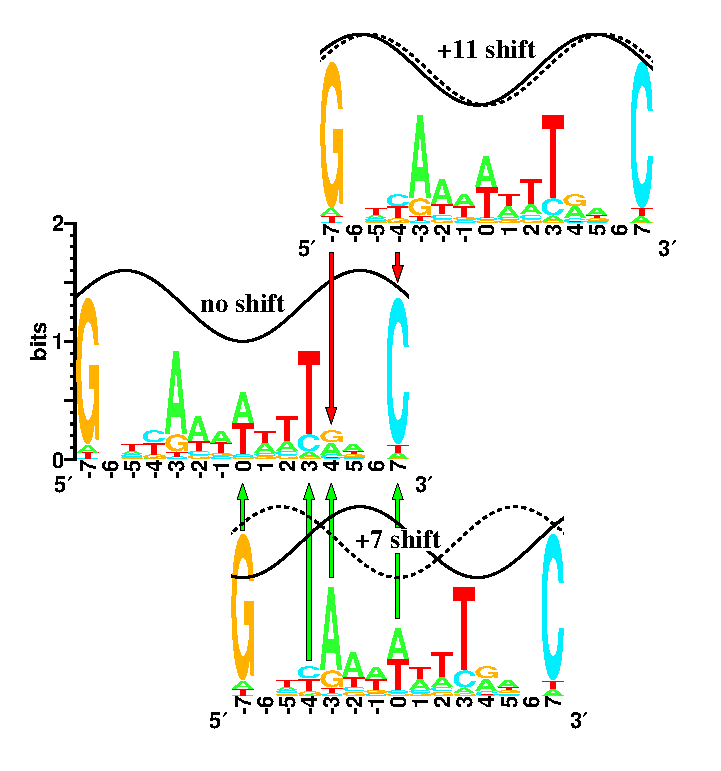
\includegraphics{selflogo.ps}}}
\begin{center}
\rotatebox{0}{\scalebox{1.00}{\includegraphics*{selflogo.ps}}}
\end{center}
% \end{makeimage}
%\vspace{-24pt}
\vspace{-28pt}
\caption{Self-similarity of Fis binding sites.}
%\begin{rawhtml}
%<br clear = all>
%\end{rawhtml}
The sequence logo for Fis
\cite{Schneider.Stephens1990,Hengen.fisinfo}
is shown three times.
The upper and lower logos are shifted $+11$ and $+7$
bases to the right (respectively) relative to the middle logo.
Dashed waves indicate the phase of the shifted site;
solid waves indicate the phase of the unshifted site.
The in-phase sine waves, with a wavelength of 10.6 bases,
show that
Fis sites shifted by 11 bases
would be on the same face of the DNA
\cite{Papp.helixrepa,Schneider.oxyr,Schneider.baseflip.2001},
while
the out-of-phase waves
of Fis sites shifted by 7 bases
indicate binding to opposite faces.
Arrows are at positions where the logo is self-similar after a shift.
Red arrows
(pointing downwards from the $+11$ shift)
mean that the contacts by Fis to the bases would interfere
because they would be on the same face of the DNA.
Green arrows
(pointing upwards from the $+7$ shift)
mean that the contacts could be simultaneous because
they are on opposite faces.
In a sequence logo,
the height of each letter is proportional to the frequency of
the corresponding base at that position in the sites,
and the height of the stack of letters represents the
sequence conservation in bits.
For clarity, the
sine waves run from 1 to 1.6 bits.
\label{fig.selflogo}
\end{figure} %%%%%%%%%%%%%%%%%%%%%%%%%%%%%%%%%%%%%%%%%%%%%%%%%%%%%%%%%%%%%%%%%%

%%% figure %%%%%%%%%%%%%%%%%%%%%%%%%%%%%%%%%%%%%%%%%%%%%%%%%%%%%%%%%%%%%%%%%%%%
\begin{figure}[ht] % b floats figure to bottom, p floats to next page, h = here
% \begin{makeimage}
%\htmlimage{transparent,thumbnail=2.0}
\begin{center}
\rotatebox{0}{\scalebox{0.90}{\includegraphics*{fismodels.ps}}}
\end{center}
\vspace{-12pt}
% \end{makeimage}
\caption{Fis binding models.}
%\begin{rawhtml}
%<br clear = all>
%\end{rawhtml}
(\textbf{a}) A single Fis dimer binding to DNA.
(\textbf{b}) Two Fis dimers binding to Fis sites separated
   by 11 base pairs.
(\textbf{c}) Two Fis dimers binding to Fis sites separated
   by 7 base pairs.
The DNA backbone is color coded:
A: green,
C: blue,
G: orange,
T: red.
The models of Fis interacting with
DNA were built using Insight II software from Biosym Technologies, Inc., on an
IRIS computer (Silicon Graphics, Inc.), and displayed with RasMol 2.5, available at
http://molbiol.soton.ac.uk/rasmol.html
or ftp://ftp.dcs.ed.ac.uk/pub/rasmol/.
The Fis
protein coordinates are those of the Protein Data Bank (http://www.rcsb.org/pdb/)
entry 1fia.
(See Materials and Methods for further details.)
\label{fig.fismodels}
\end{figure} %%%%%%%%%%%%%%%%%%%%%%%%%%%%%%%%%%%%%%%%%%%%%%%%%%%%%%%%%%%%%%%%%%

%%% figure %%%%%%%%%%%%%%%%%%%%%%%%%%%%%%%%%%%%%%%%%%%%%%%%%%%%%%%%%%%%%%%%%%%%
\begin{figure}[ht] % b floats figure to bottom, p floats to next page, h = here
% \begin{makeimage}
%\htmlimage{thumbnail=1.4,antialias} 
% \rotatebox{-90}{\scalebox{0.54}{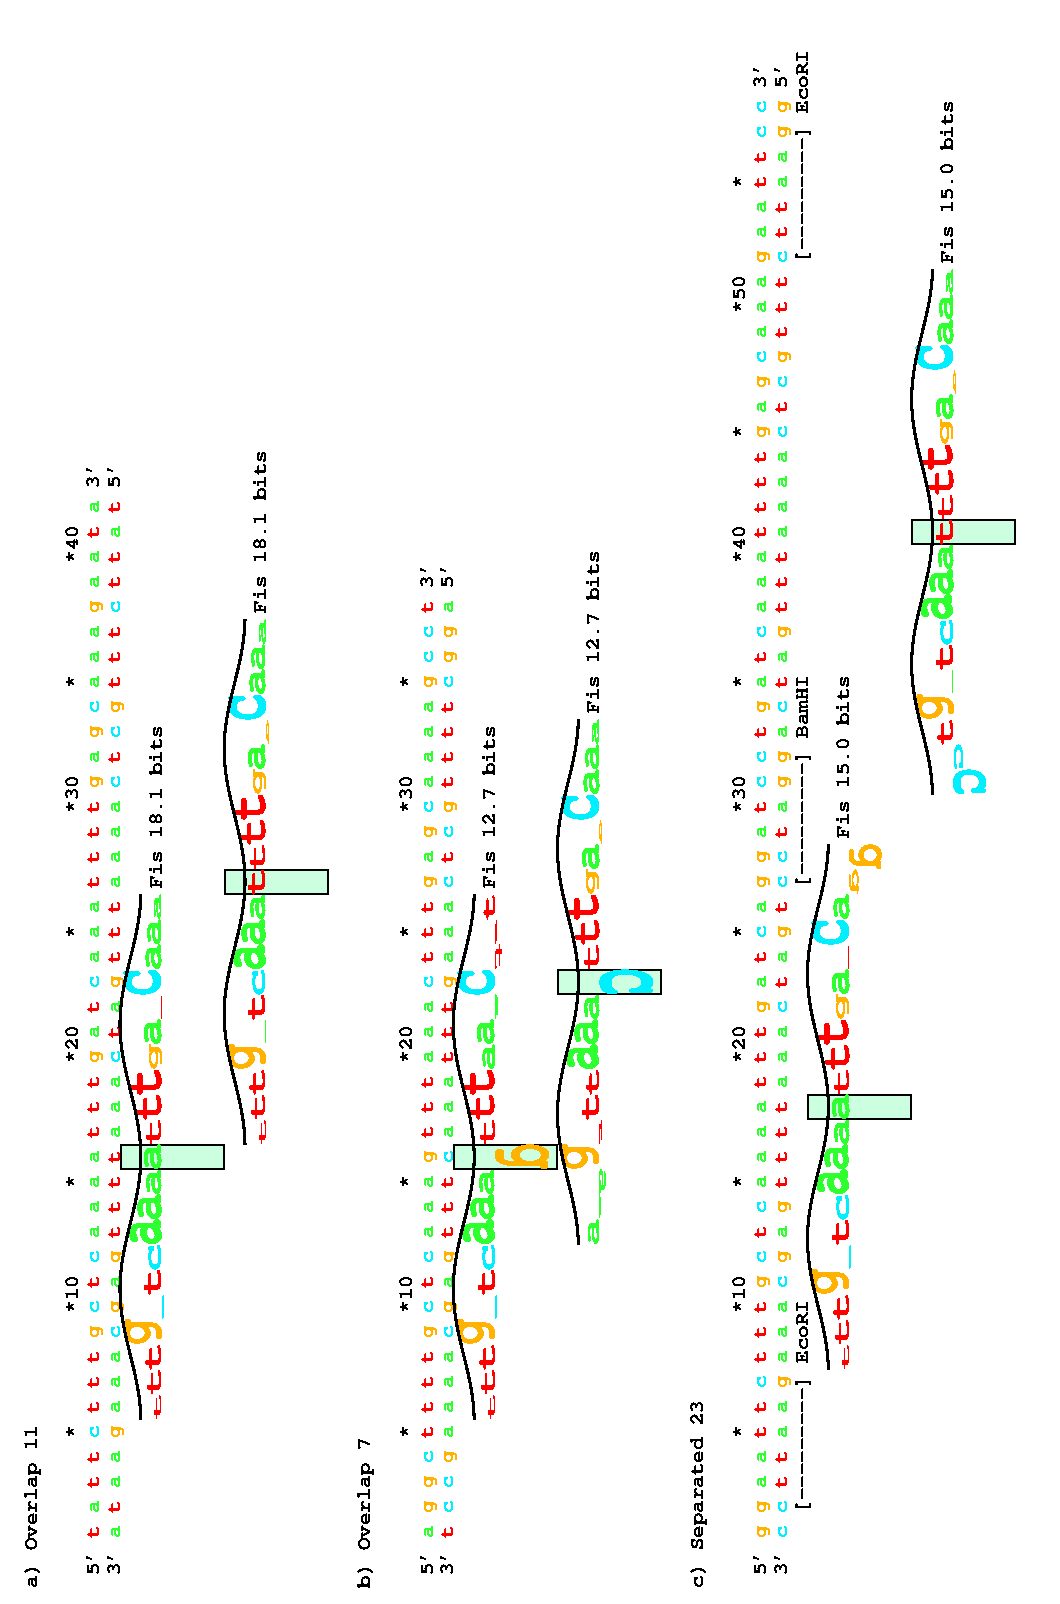
\includegraphics{overlap.ps}}}
% \rotatebox{-90}{\resizebox{!}{7.5in}{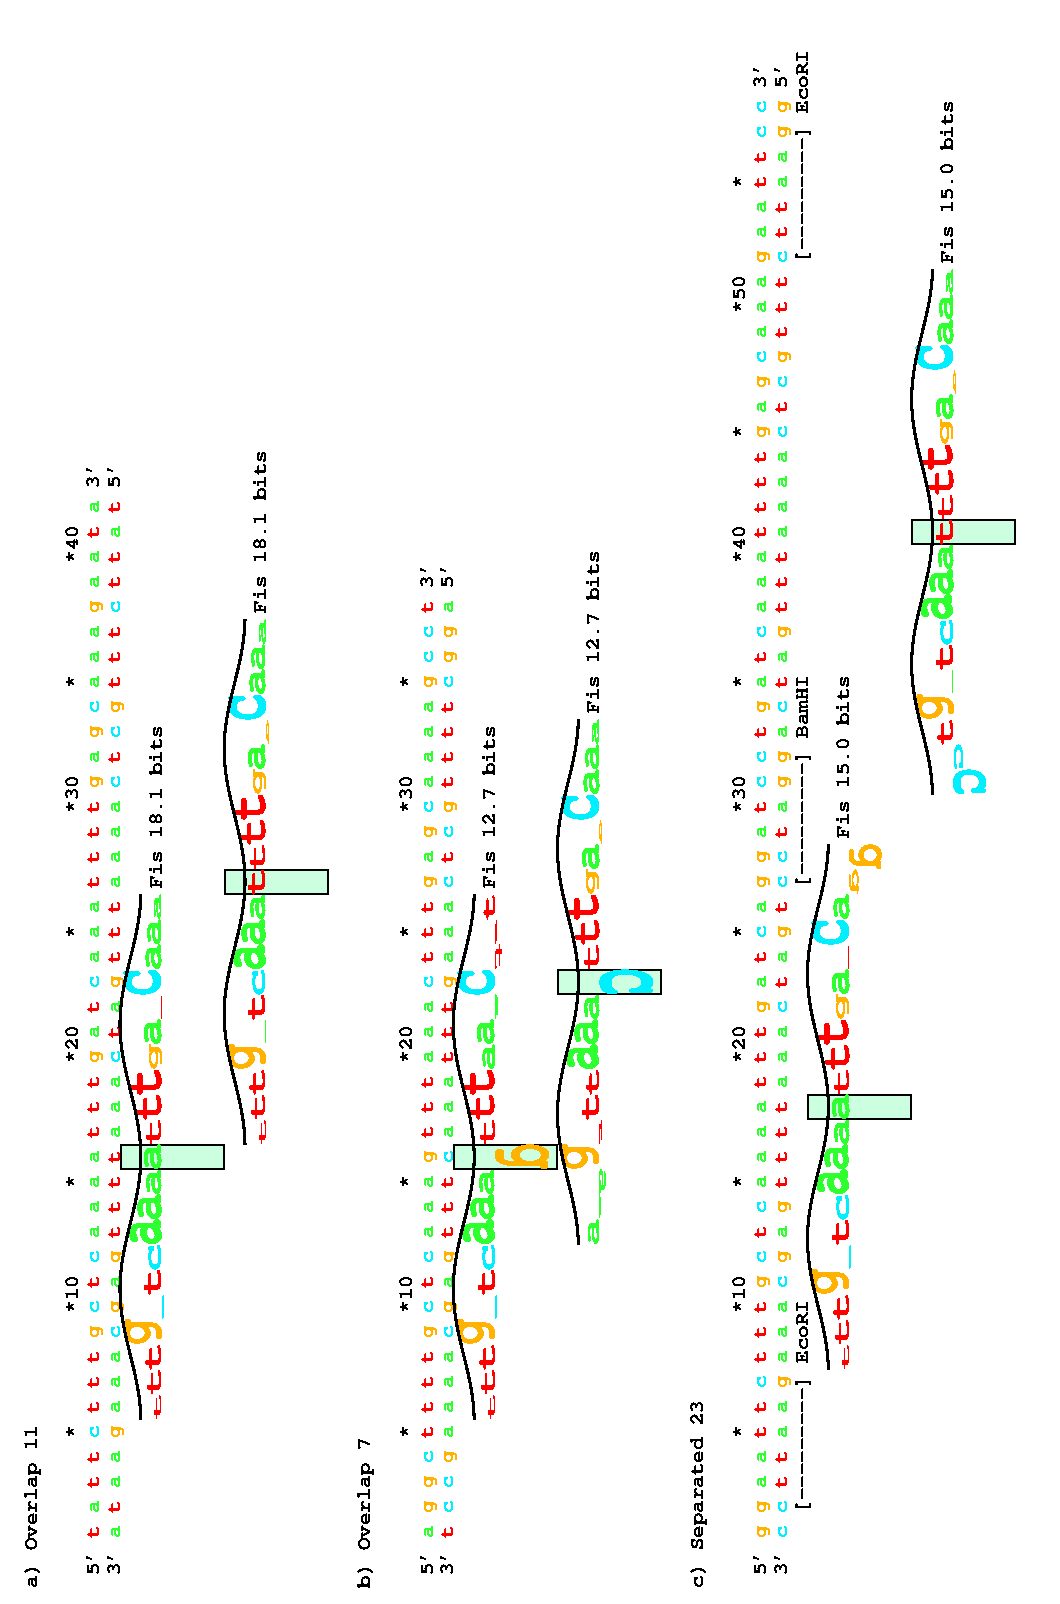
\includegraphics{overlap.ps}}}
% very cool!  One can make the figure fit the current page width!!
\rotatebox{-90}{\resizebox{!}{\textwidth}{\includegraphics*{overlap.ps}}}
% \end{makeimage} 
\caption{Oligonucleotide design of overlapping and separated Fis binding sites.}
%\begin{rawhtml}
%<br clear = all>
%\end{rawhtml}
The predicted Fis sites are shown by sequence walkers
floating below each self-complementary DNA sequence
\cite{Schneider.walker,Hengen.fisinfo}.
In a walker, the vertical
green box marks the zero base of the binding site.
The box also shows the vertical scale, with the upper edge being at $+2$ bits
and the lower edge being at $-3$ bits.
The height of each letter
is determined from the bit value
in the
individual information weight matrix
\cite{Schneider.Ri,Schneider.walker,Hengen.fisinfo}.
Negative weights are represented by drawing the letter
upside-down
and placing it below the zero bit level.
To indicate predicted relative orientations,
the peaks of sine waves correspond to where Fis
would bind into the major groove.
Three DNAs were designed, each having
two Fis sites spaced 11, 7 and 23 bases apart.
Design details are given in Materials and Methods.
The total strength of a site is the sum of the information weights for each
base.
The $18.1$ bit Fis sites are
3.4
standard deviations
higher than the average Fis site
in natural sequences \cite{Hengen.fisinfo,Schneider.Ri}.
The
$12.7$ and $15.0$ bit sites are
1.6 and 2.4
standard deviations above average, respectively.
\label{fig.sequences-overlap}
\end{figure} %%%%%%%%%%%%%%%%%%%%%%%%%%%%%%%%%%%%%%%%%%%%%%%%%%%%%%%%%%%%%%%%%%

%%% figure %%%%%%%%%%%%%%%%%%%%%%%%%%%%%%%%%%%%%%%%%%%%%%%%%%%%%%%%%%%%%%%%%%%%
\begin{figure}[ht] % b floats figure to bottom, p floats to next page, h = here
% \begin{makeimage}
%\htmlimage{transparent,thumbnail=1.4,antialias} 
% \rotatebox{90}{\scalebox{0.54}{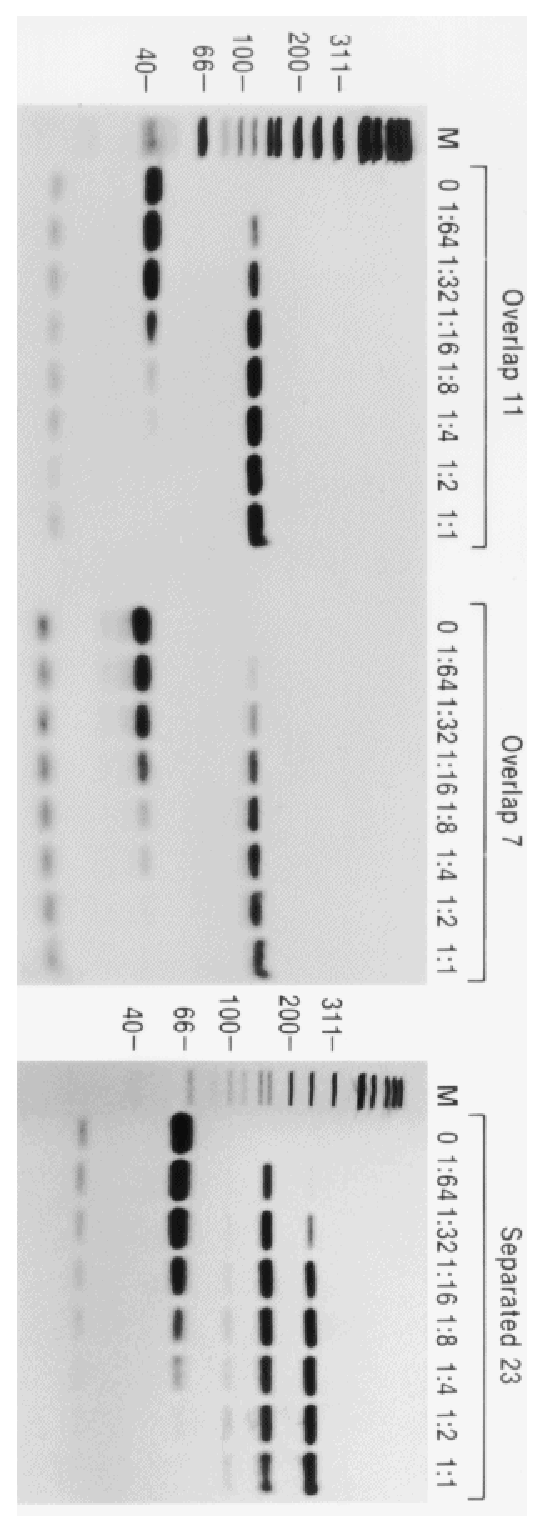
\includegraphics{gel-overlap.ps}}}
% very cool!  One can make the figure fit the current page width!!
\rotatebox{90}{\resizebox{!}{\textwidth}{\includegraphics*{gel-overlap.ps}}}
% \end{makeimage} 
\caption{Mobility shift experiments for 11 and 7 base pair overlapping
and 23 base pair separated Fis sites.}
%\begin{rawhtml}
%<br clear = all>
%\end{rawhtml}
\label{fig.gel-overlap}
Each lane contains increasing
concentrations of Fis protein,
beginning with
no Fis, Fis diluted 1 to 64, etc.
The 1:1 dilution was at 2200 nM Fis.
This concentration was chosen intentionally so that with
the 1 nM of DNA used in this experiment,
the protein/DNA ratio was 2-fold higher
than that
needed to strongly shift
DNA containing
the 8.9 bit wild-type \emph{hin} distal Fis site
\cite{Bruist1987}.
The sequences are given in \fig{fig.sequences-overlap}.
Marker lanes (M) contain 10 ng of biotinylated $\phi$X174
\emph{Hinf}I digested DNA standards (Life Technologies, Inc.).
Sizes are indicated in bp.
The lowest band in most lanes of the figure is single-stranded
oligonucleotide DNA.  In the ``Separated 23'' experiment,
at high concentrations, Fis proteins are apparently able to
capture the single-stranded DNA
when it has folded into a hairpin.
This produces a faint band near the 100 bp marker.
%
%*******************************************************************************
% b) Lanes either did not ($-$) or did ($+$) contain 2200 nM Fis.
% The $\Phi$66 lanes contained
% two co-migrating isolated 66 bp $\Phi$X174
% \emph{Hinf}I digested DNA standards (Life Technologies, Inc.). \\
%*******************************************************************************
%From pnh@ncifcrf.gov Fri Aug  2 11:50 EDT 1996
%From: Paul N Hengen <pnh@ncifcrf.gov>
%Subject: Re: Kostrewa1992
%To: toms@ncifcrf.gov (Tom Schneider)
%Date: Fri, 2 Aug 1996 11:55:27 -0400 (EDT)
%
%> Paul:  Kostrewa1992 (page 224) did indeed talk about the AT in the center and
%> even about the YR conservation.  Check it out.  I have inserted references to
%> them.  Missing this would have been a serious mistake.  (We get to sock it to
%> them for the things they said about Fis being atypical just before that
%> passage ;-)  Tom
%
%Tom:
%
%I also checked on the Fis/DNA concentration that I used compared to
%Bruist1987. This should read 2-fold higher concentration rather than
%2.2-fold higher. My notes of 15 December 1995 say that Bruist1987 used
%0.2 nM DNA and 229 nM Fis in their highest ratio. Since I used 1 nM
%of DNA and 2200 nM Fis, it is 2-fold higher.
%
%1145 Fis/DNA versus 2200 Fis/DNA = 1.92-fold
%
%We can add into that sentence...  "the amount of Fis we used was 2-fold higher
%than that needed to shift 100% of DNA containing the wild-type Hin distal Fis
%site (9.2 bits) (Bruist1987)."
%
%-Paul.
\end{figure} %%%%%%%%%%%%%%%%%%%%%%%%%%%%%%%%%%%%%%%%%%%%%%%%%%%%%%%%%%%%%%%%%%

%%% figure %%%%%%%%%%%%%%%%%%%%%%%%%%%%%%%%%%%%%%%%%%%%%%%%%%%%%%%%%%%%%%%%%%%%
\begin{figure}[ht] % b floats figure to bottom, p floats to next page, h = here
% \begin{makeimage}
%\htmlimage{transparent,thumbnail=1.4,antialias} 
% \rotatebox{-90}{\scalebox{0.54}{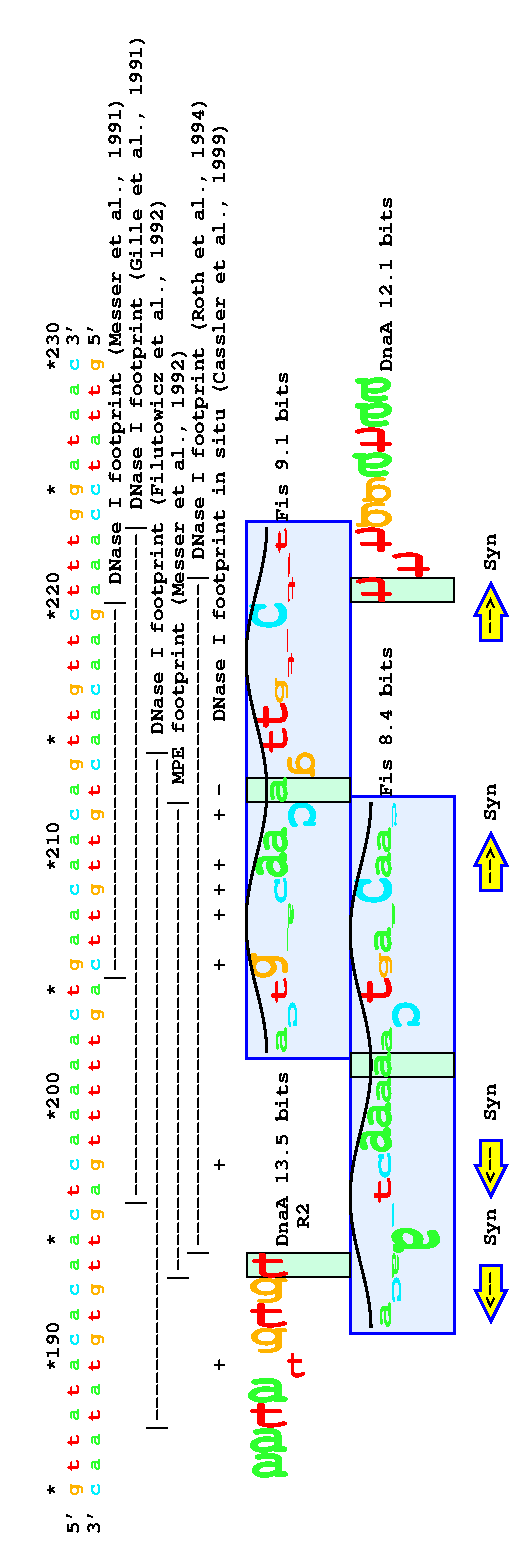
\includegraphics{oric.ps}}}
% very cool!  One can make the figure fit the current page width!!
\rotatebox{-90}{\resizebox{!}{\textwidth}{\includegraphics*{oric.ps}}}
% \end{makeimage} 
\caption{Positions of Fis and DnaA sites at the \emph{E. coli oriC}
shown by sequence walkers.}
%\begin{rawhtml}
%<br clear = all>
%\end{rawhtml}
Sequence data are from GenBank accession K01789
\cite{Messer.Schaller1979}.
The horizontal dashes below the sequence
represent regions protected by Fis.
% Note: The footprints were placed according to the
% published results of those papers below:
% 206 to 220 \cite{Messer1991},
% 197 to 223 \cite{Gille1991},
% 188 to 214 \cite{Filutowicz1992},
% 194 to 212 \cite{Messer1992},
% 195 to 220 \cite{Roth1994}.
Locations of DnaA sites are from
Messer \emph{et al.}
\cite{Messer1991}
and Fis footprint data are from
% \cite{Messer1991,Gille1991,Filutowicz1992,Messer1992,Roth1994,Cassler.Leonard1999}.
Messer \emph{et al.} \cite{Messer1991},
Gille \emph{et al.} \cite{Gille1991},
Filutowicz \emph{et al.} \cite{Filutowicz1992},
Messer \emph{et al.} \cite{Messer1992},
Roth \emph{et al.} \cite{Roth1994},
and
Cassler \emph{et al.} \cite{Cassler.Leonard1999}.
The asymmetric
DnaA individual information matrix was created from 27 experimentally
demonstrated DnaA binding sites
\cite{Schneider.baseflip.2001}.
DNA synthesis start sites are indicated by yellow arrows and `Syn'
\cite{Seufert.Messer1987};
however start sites 
have also been mapped to the left side of \emph{oriC}
\cite{Fang.O'Donnell1999}.
Blue boxes mark two Fis sites separated by 11 bases.
%Fis sites with positive individual information
%are marked from $-7$ to $+7$ but evaluated from $-10$ to $+10$
%according to the matrix.
DnaA site directionality is indicated by letters turned
sideways in the direction that
DnaA binds \cite{Schneider.walker}.
\label{fig.oriC}
\end{figure} %%%%%%%%%%%%%%%%%%%%%%%%%%%%%%%%%%%%%%%%%%%%%%%%%%%%%%%%%%%%%%%%%%

%%% figure %%%%%%%%%%%%%%%%%%%%%%%%%%%%%%%%%%%%%%%%%%%%%%%%%%%%%%%%%%%%%%%%%%%%
\begin{figure}[ht] % b floats figure to bottom, p floats to next page, h = here
% \begin{makeimage}
%\htmlimage{transparent,thumbnail=1.4,antialias}
\scalebox{0.69}{\includegraphics*{fisori.ps}}
% \end{makeimage}
\caption{\emph{E. coli oriC} can bind only one Fis molecule
at a time between DnaA sites R2 and R3.}
A. Design of wild-type and mutated Fis sites from
\emph{E. coli} \emph{oriC}.
Four hairpin oligos were designed and designated
\textbf{nn},
\textbf{no},
\textbf{on}
and
\textbf{oo}
where \textbf{n} means no site
because of engineered mutations
(pink boxes, with information less than zero)
and \textbf{o} means that there is
a complete wild-type origin Fis site
(green boxes, with positive information).
For example,
\textbf{no} contains only the Fis site closest to R3 on the right side.
\\
B.  Gel mobility shift assay with \emph{oriC} sites using the oligos
shown in part A at a concentration of 10 nM each.
Fis concentrations were 0, 30, 100, 300 and 1000 nM.
u: unbound DNA;
b: Fis bound DNA.
%\begin{rawhtml}
%<br clear = all>
%\end{rawhtml}
\label{fig.oriCexperiment}
\end{figure} %%%%%%%%%%%%%%%%%%%%%%%%%%%%%%%%%%%%%%%%%%%%%%%%%%%%%%%%%%%%%%%%%%

%%% figure %%%%%%%%%%%%%%%%%%%%%%%%%%%%%%%%%%%%%%%%%%%%%%%%%%%%%%%%%%%%%%%%%%%%
\begin{figure}[ht] % b floats figure to bottom, p floats to next page, h = here
% \begin{makeimage}
%\htmlimage{transparent,thumbnail=1.4,antialias}
% very cool!  One can make the figure fit the current page width!!
% \rotatebox{0}{\resizebox{!}{\textwidth}{\includegraphics{norgate.eps}}}
% can't use \textwidth on this figure :-(
% \end{makeimage}
%
%\begin{center}
% \scalebox{1.25}{\includegraphics*{norgate.eps}}
%\end{center}
% revised 2003 oct 3 for portrait mode:
\vspace{-10 cm}
\hspace{-2 cm}
\scalebox{1.00}{\includegraphics*{norgate.eps}}
\vspace{-11 cm}
\caption{NOR Gate molecular computer.}
An activator protein molecule \textbf{A} (green plus)
binds to a DNA molecule at position \textbf{a}.
When the activator binds, it turns on the promoter for gene \textbf{D}.
Two repressor protein molecules
\textbf{R1} and \textbf{R2} (red circle and red hexagon respectively)
bind to DNA at positions \textbf{r1} and \textbf{r2}.
Binding to either \textbf{r1} or \textbf{r2}
interferes with binding by \textbf{A},
so the activator can only bind when the two repressors are absent.
Assigning the presence of a molecule as `1' or `true' and the absence as `0'
or `false',
then \textbf{D = R1 NOR R2}.
By connecting such NOR gates together, any computer circuit can be built.
%\begin{rawhtml}
%<br clear = all>
%\end{rawhtml}
\label{fig.norgate}
\end{figure} %%%%%%%%%%%%%%%%%%%%%%%%%%%%%%%%%%%%%%%%%%%%%%%%%%%%%%%%%%%%%%%%%%

%*******************************************************************************

\clearpage % force figures out

\newpage

% PROPOSED COVER FIGURE
% This is not really a figure in the paper, so don't treat it as one -
% the figure mechanism is blocked.

$\;$ % fool LaTex to make space

\vspace{120 pt}

%%% figure %%%%%%%%%%%%%%%%%%%%%%%%%%%%%%%%%%%%%%%%%%%%%%%%%%%%%%%%%%%%%%%%%%%%
%\begin{figure}[ht] % b floats figure to bottom, p floats to next page, h = here
% \begin{makeimage}
%\htmlimage{transparent,thumbnail=1.4,antialias}
%\framebox[6 in][l]{
%\mbox{
\begin{center}
\scalebox{1.00}{\includegraphics*{cover.ps}}
\end{center}
%}
%}
% \end{makeimage}
%\caption{
Proposed cover figure.
%}
``Fis binding sites form a
bi-stable
flip-flop in the
\emph{Escherichia coli}
origin of replication.''
%\begin{rawhtml}
%<br clear = all>
%\end{rawhtml}
%\label{fig.cover}
%\end{figure} %%%%%%%%%%%%%%%%%%%%%%%%%%%%%%%%%%%%%%%%%%%%%%%%%%%%%%%%%%%%%%%%%%

% ******************************************************************************

\end{document}
%]]text

%*******************************************************************************
